% !TEX root = ../thesis.tex
\chapter{Behaviours of Evaluation Engines}
\label{sec:behaviours}

Based on the definitions in \cref{sec:definitions} we will now look at different schedules of evaluation engines and compare them.
This is done in multiple steps: starting with a small subset of allowed schedules and functions and iteratively adding more complex cases.

For the comparision we will use timed transducers from \cref{sec:definitions:timed_transducer}.
To do this the notion of a run of an evaluation engine is not sufficient: transducers describe a relationship between inputs and outputs, runs describe stepwise generation of internal and output events.
Therefore the \emph{behaviour} of a run is defined, which maps a run to relationship between inputs and outputs.

\begin{definition}[name = Behaviour of a Run]\label{def:behaviour_run}
  Let \(r\) be a run of an evaluation engine.
  The behaviour \(\beta_r\) of it is a timed transducer: A set of tuples of timed sequences.
  It is calculated as follows:
  \begin{enumerate}
    \item Let \(\beta_r = \emptyset\) and \(r_p\) an empty prefix of \(r\).
    \item Remove the prefix  from \(r\), where the first transition consumes an input upto but not including the next transition where an input is consumed, and append it to \(r_p\).
    \item Select the sequence of all output events \(O_p\) (which is possible empty) that are produced at any step in \(r_p\).
    \item Select the sequence of all input events \(E_p\) that are consumed at any step in \(r_p\).
    \item Add the tuple \((E_p,O_p)\) to \(\beta_r\).
    \item Goto step 2 if \(r\) is not empty, else terminate.
  \end{enumerate}

  Stated simple the run is chopped into pieces, where each piece begins with the consumption of an input events and ends before the next input is consumed.
  The pieces are then merged from left to right: First take all inputs and outputs consumed and produced upto the current piece and add them to the behaviour, then merge the current piece with the next and repeat.
\end{definition}

\begin{exmp}[name = Construction of a Behaviour]\label{exmp:construction_of_behaviour}
  In \cref{table:chap5:sec_behaviour:construction_run} it is shown how a behaviour is built from a run.
  The run ist denoted only by its transitions, events are labeled based on their type: \(e_i\) are external (read: input) events, \(i_i\) are internal events and \(o_i\) are output events.
  Parts of the run in the same color are the transitions that end up in the same piece when applying the constuction algorithm.
  The tuples show how the sequence of input and output events from the pieces are extracted.
  The behaviour of the run is the set of the tuples.

  \begin{table}
    \renewcommand{\arraystretch}{1.5}
    \begin{tabular}{llllll}
      Run    & \multicolumn{5}{l}{\textcolor{red}{\(    (\{e_1\},\{i_1\})\ (\{i_1\},\{i_2\})\ (\{i_1,i_2\},\{o_1\})\ \)}\textcolor{Cyan}{\((\{e_2\},\{i_3\})\ (\{i_2,i_3\},\{o_2\})\)}\(\hookleftarrow\)} \\
      & \multicolumn{5}{l}{\hspace{1em}\textcolor{Cyan}{\(    (\{i_3\},\{o_3\})\ \)}\textcolor{OliveGreen}{\((\{e_3\},\{i_4\})\ \)}\textcolor{BurntOrange}{\((\{e_4\},\{i_5\})\ (\{i_4,i_5\},\{o_4\})\)}} \\
      Tuples & \textcolor{red}{\((e_1,o_1)\)} & \textcolor{Cyan}{\((e_1e_2,o_1o_2o_3)\)} & \textcolor{OliveGreen}{\((e_1e_2e_3,o_1o_2o_3)\)} & \textcolor{BurntOrange}{\((e_1e_2e_3e_4,o_1o_2o_3o_4)\)} \\
    \end{tabular}
    \caption{Example how the behaviour of a run is constructed}\label{table:chap5:sec_behaviour:construction_run}
  \end{table}
\end{exmp}

The behaviour of a run is a timed transducer since all events have timestamps and all consumed events are strictly ordered by their timestamp, since inputs to an evaluation engine are required to be ordered by their timestamp.

Since the behaviour encodes the relationship between inputs and outputs a run produces it provides the foundation to reason about equivalence between different runs and whole evaluation engines.

\begin{definition}[name=Equivalence of Runs]\label{def:equivalence_runs}
  Two runs are called equivalent if their behaviour is observational equivalent.
\end{definition}

Now we can define when two evaluation engines are called equivalent based on their runs

\begin{definition}[name=Equivalence of Evaluation Engines]\label{def:equivalence_eval_engine}
  Two evaluation engines are called equivalent, if for every run that one can produce there is an observational equivalent run in the other.
\end{definition}

\section{Schedules Without Timing Functions}
\label{sec:behaviours:without_timing}

For a first step we specify and compare behaviours of different approaches to evaluate \gls{tessla} specifications without timing functions.
Without timing functions all nodes work only on values or the presence of events and will emit exactly one event at every computation, either a normal or a progress event.
This leads to behaviours that can be easily reason about, as seen in the next sections.

All systems to evaluate \gls{tessla} specifications we will look at are based on the described structure in \cref{sec:definitions:eval_engine}.
While there are other approaches to evaluation, a \gls{dag} based approach seems to fit most naturaly and focusing on one structure makes comparing systems easier.

Let's recap and summarize how an evaluation engine performs its computation.
Each evaluation engine will work in steps, where each step is synonymous with an index in the run of the system.
Therefore at each step one enabled node is scheduled to perform its operation, represented as the transition in the run.
The transition will encode one of the following three things that can happen:

\begin{itemize}
  \item The next external event (external events have to be totally ordered by their timestamp) can be consumed by a source in the \gls{dag}, which generates internal events, that are propagated to its children.
  \item An internal node, which has at least one new input buffered on all of its input queues, can perform its computation and generate a new internal event, which is propagated to the children of that node.
  \item An output node, which has at least one new input buffered on all of its input queues, can produce a new output.
\end{itemize}

Evaluation engines are free in the way they are scheduling their nodes, only limited by causality (no event can be consumed before it's produced), which is guaranteed by the enabledness criteria.
In the following evaluation engines are classified by their scheduling approaches.

\subsection{Greedy Evaluation Engines}
\label{sec:behaviours:without_timing:greedy}

The first class of evaluation engines are called greedy.

\begin{definition}[name = Greedy schedule]\label{def:greedy_schedule}
  A schedule of an evaluation engine built by the following steps is called \emph{greedy}.
  \begin{enumerate}
    \item Select all nodes that are no sources, let their count be \(i\)
    \item Label them with unique natural numbers from \([1,i]\) in reverse topological order
    \item Label the remaining nodes with unique natural numbers bigger than \(i\)
    \item Schedule the enabled node with the lowest label first
  \end{enumerate}

  We also call an evaluation engine greedy if we mean it's run with a greedy schedule.
\end{definition}

Obviously for many \glspl{dag} there is no unique reverse topological order, therefore one can be chosen by the evaluation engine.
We will show in \cref{sec:behaviours:equivalence_without_timing:greedy} that all topological orders will produce observational equivalent behaviours.

The greedy schedule ensures that no node is scheduled which has a successor that can be scheduled, therefore events are \emph{pushed} through the \gls{dag} towards an output node as fast as possible.
As shown in \cref{sec:behaviours:without_timing:greedy:is_fair} any schedule built like this is fair.

Greedy evaluation engines offer a good start to reason about behaviours and will be used as a comparision for all other evaluation engines.

\begin{definition}[name = Valid Evaluation Engines]\label{def:valid_eval_engine}
  An evaluation engine is called \emph{valid} if it is equivalent to a greedy evaluation engine.
\end{definition}


\begin{figure}
  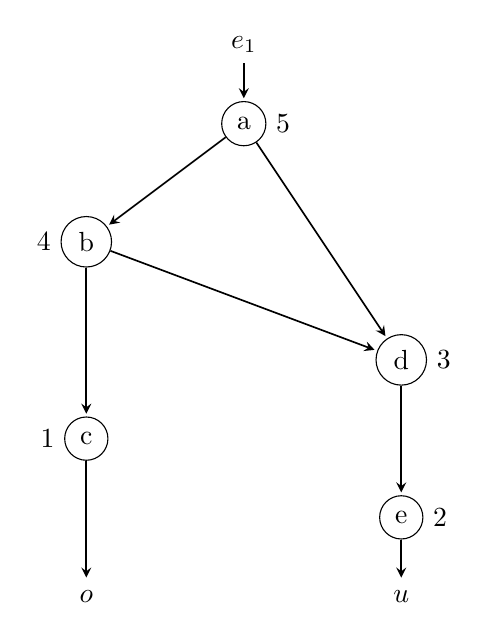
\begin{tikzpicture}
    [pre/.style={<-,shorten <=1pt,>=stealth,semithick}]
    \node (s) at (2,5) {\(e_1\)};
    \node [shape=circle,draw=black] (a) [label=right:5] at (2, 4) {a}
      edge [pre] (s);
    \node [shape=circle,draw=black] (b) [label=left:4] at (0,2.5) {b}
      edge [pre] (a);
    \node [shape=circle,draw=black] (c) [label=left:1] at (0,0) {c}
      edge [pre] (b);
    \node [shape=circle,draw=black] (d) [label=right:3] at (4,1) {d}
      edge [pre] (a)
      edge [pre] (b);
    \node [shape=circle,draw=black] (e) [label=right:2] at (4,-1) {e}
      edge [pre] (d);
    \node (o1) at (0,-2) {\(o\)} edge [pre] (c);
    \node (o2) at (4,-2) {\(u\)} edge [pre] (e);
  \end{tikzpicture}
  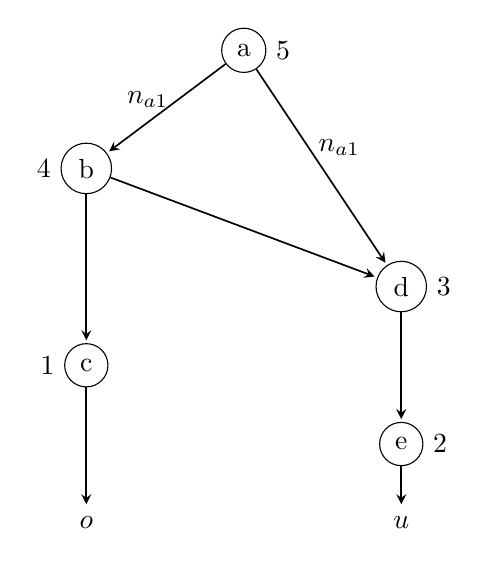
\begin{tikzpicture}
    [pre/.style={<-,shorten <=1pt,>=stealth,semithick}]
    \node [shape=circle,draw=black] (a) [label=right:5] at (2, 4) {a};
    \node [shape=circle,draw=black] (b) [label=left:4] at (0,2.5) {b}
      edge [pre] node[align=left,left,pos=0.6] {\(n_{a1}\)} (a);
    \node [shape=circle,draw=black] (c) [label=left:1] at (0,0) {c}
      edge [pre] (b);
    \node [shape=circle,draw=black] (d) [label=right:3] at (4,1) {d}
      edge [pre] node[align=right,right,pos=0.6] {\(n_{a1}\)} (a)
      edge [pre] (b);
    \node [shape=circle,draw=black] (e) [label=right:2] at (4,-1) {e}
      edge [pre] (d);
    \node (o1) at (0,-2) {\(o\)} edge [pre] (c);
    \node (o2) at (4,-2) {\(u\)} edge [pre] (e);
  \end{tikzpicture}
  \caption{Visualization of a simple evaluation engine with a greedy schedule.}
  \label{fig:chap5:sec_greedy:visual_dag}
\end{figure}

\Cref{fig:chap5:sec_greedy:visual_dag} visualizes a greedy evaluation engine.
It shows two \glspl{dag} representations of an evaluation engine  where the nodes \(a\) to \(e\) are labeled in a reversed topological order and \(o\) and \(u\) represents two output streams.
The left system is in its initial state and an input event \(e_1\) is present and can be consumed by the input node \(a\).
When a node is chosen to compute by the scheduler, only node \(a\) is enabled, therefore it is scheduled.
The right system is the representation of the next step: node \(a\) has consumed the external event and produced an internal event \(n_{a1}\), which is propagated to all its children: nodes \(b\) and \(d\).
In the next step node, \(b\) would be scheduled, because it has the lowest number of any node that can compute (actually it's the only node that can compute at all, because \(d\) has to wait for the event from \(b\)).
After \(b\) is scheduled, it would produce the internal event \(n_{b1}\) which would then be distributed to nodes \(c\) and \(d\).

The complete run of the greedy engine for one input is the following, where the states are omitted:

\begin{align*}
  \langle
    (\lambda,                             s_0),
    ((\{ n_{a1}         \}, \{n_{b1}\}),  s_1),
    ((\{ n_{b1}         \}, \{o_1\}),     s_2),\\
    ((\{ n_{a1}, n_{b1} \}, \{n_{d1}\}),  s_3),
    ((\{ n_{d1}         \}, \{u_1\}),     s_4)
  \rangle
\end{align*}

If there were more than one input event, at this point node \(a\) would be scheduled again.
It would consume the next external event and the following nodes would be scheduled in the same order as before, extending the run in an obvious way.

\subsubsection{Fairness of Greedy Schedules}
\label{sec:behaviours:without_timing:greedy:is_fair}

It remains to show that greedy schedules are fair.

\begin{lemma}[name = Greedy Schedules are Fair]\label{lemma:greedy_schedules_are_fair}
  Any greedy schedule is fair.
\end{lemma}

\begin{proof}
  Let \(a\) be a node with the label \(n\), which is enabled at step \(i\) and is no source.
  Because evaluation engines can only contain a finite number of nodes there can only be a finite number of enabled nodes with a smaller label than \(n\).
  Because of \cref{lemma:finiteness_enabledness}, all nodes with a smaller label than \(n\) will become disabled after a finite number of steps.
  Let that number be \(j\).
  The only way new events could enter the system are through sources, but they have bigger labels than \(n\), as by the definition of the schedule, and therefore can't be scheduled before \(n\).
  Because of \cref{lemma:enabled_till_scheduled}, \(a\) will still be enabled after these steps.
  So \(a\) is the enabled node with the lowest label at step \(i + j\) and therefore will be scheduled.

  Now let \(a\) be a source.
  Sources are only scheduled when no internal node is enabled since they are labeled with higher numbers than all internal nodes.
  Based on the same reasoning as in the first case at some point all internal nodes will become disabled, therefore a source node has to be scheduled.
  This source can either be \(a\) or another source, recall that only one source is enabled at any time because of the environment of an evluation engine.
  If another source was scheduled, after a finite amount of steps all internal nodes will have to become disabled again.
  Since finite traces are evaluated at some point either the trace will end without ever feeding an input to \(a\), then \(a\) will never be enabled, or at some point \(a\) will receive an external event.
  When \(a\) receives an external event, it will be the only enabled source, else no input would be fed to an input at that step.
  Therefore \(a\) will be scheduled the next time no internal nodes are enabled.
\end{proof}


\subsection{Fair Evaluation Engines}
\label{sec:behaviours:behaviour_without_timing:fair}

Obviously greedy schedules are only a small subset of all fair schedules.
As the next step we will look at the rest of them.

\begin{definition}[name = Fair Evaluation Engines]\label{def:fair_evaluation_engines}
  A fair evaluation engine is one with a fair schedule.
\end{definition}

In contrast to a greedy evaluation engine a fair one has no fixed schedule, meaning that at each step any enabled node can be scheduled.
Therefore predecessors of enabled nodes can perform multiple computations before their children are scheduled and events are not \emph{pushed} through the \gls{dag} as fast as possible.

The difference between greedy and fair schedules are similar to the ones of synchronous and asynchronous transducers: A greedy schedule will ensure that outputs are produced as fast as possible while a fair can \emph{delay} the outputs by consuming multiple inputs first and scheduling internal nodes multiple times before scheduling an output node.
But note that there is an important difference between synchronous transducers and the behaviour of a greedy evaluation engine: A greedy evaluation engine can produce multiple events at every step.

\section{Equivalence of Different Schedules Without Timing Functions}
\label{sec:behaviours:equivalence_without_timing}

The behaviour of a run of an evaluation engine with a given schedule allows us to reason about equivalence.

As by \cref{def:valid_eval_engine} any evaluation engine has to be equivalent to a greedy one to be valid.

The equivalence is shown in two steps: first in \cref{sec:behaviours:without_timing:greedy} it is shown, that all possible greedy engines for a specification are equivalent, so there is only one valid evaluation for a specification over a fixed input.
Afterwards in \cref{sec:behaviours:equivalence_without_timing:greedy_fair} it is shown that any fair evaluation engine is equivalent to a greedy one.


\subsection{Equivalence of Greedy Systems}
\label{sec:behaviours:equivalence_without_timing:greedy}

When given a series of input events, two greedy evaluation engines for a specification with different schedules will have different runs.
But both will produce all outputs that can be produced after consuming one specific input before the next input is consumed as reasoned in \cref{sec:behaviours:without_timing:greedy}.
Also both runs will obviously have the same length (both engines are the same \gls{dag}, so they have the same number of nodes), let that length be \(l\).

To proof the equivalence of both engines we can prove the equivalence of their runs.
To show the equivalence it is shown that two runs \(r_1\) and \(r_2\) of two evaluation engines based on the same graph but with a different greedy schedule can always be reordered to become closer while preserving observational equivalence.
If such a closer run always exist, we will show that the run with closeness \((l, 0)\) to \(r_1\), which has to be \(r_1\) itself, is also observational equivalent to \(r_2\).

\begin{theorem}[name = Equivalence of Different Greedy Evaluation Engines]\label{theorem:equivalence_greedy_eval_engines}
  Two greedy evaluation engines for a specification with different schedules are equivalent.
\end{theorem}


\begin{proof}\label{proof:equiv_greedy_engines}
  Let \(r_1, r_2\) be the runs of two greedy evaluation engines for the same specification which received the same inputs.
  Because each \gls{tessla} specification contains only a finite amount of functions and works on finite traces, the runs also have to be finite.

  If the two runs aren't equal, they must have a closeness which is smaller than \((l, 0)\).
  Let \([r_2]\) be the set of all runs that are observational equivalent to \(r_2\).
  If \(r_1\) is in this set, we would be done.
  Let's assume that \(r_1\) is not in the set.
  Therefore all runs in the set have to have a smaller closeness than \((l,0)\) to \(r_1\), since the only run with a closeness of \((l,0)\) to another run is the run itself.
  Select one run \(r_2' \in [r_2]\) which has the biggest closeness to \(r_1\).
  Let \((d,k) = \delta(r_1, r_2')\).

  This means that at step \(d\) the run \(r_2'\) has taken a different transition than run \(r_1\).
  Let the transitions the runs have taken be \(\tau_1\) for \(r_1\) and \(\tau_2\) for \(r_2'\).
  Run \(r_2'\) will take transition \(\tau_1\) at step \(d+k\) (as per the definition of the closeness).
  Obviously the two transitions have to be independent of each other, else they couldn't have been taken in different order by the two runs.

  If \(k > 1\) there will be a transition \(\tau_2' \neq \tau_1\) which is taken by the run \(r_2'\) at step \(d+(k-1)\).
  While this transition \(\tau_2'\) must also be taken in the first run as per \cref{lemma:enabled_till_scheduled}, it's not possible, that it was taken before \(\tau_1\), beause then the two runs wouldn't have been the same upto the point where \(\tau_1\) was taken.
  Therefore \(\tau_1\) has to be independent of \(\tau_2'\), and because \(\tau_2'\) was scheduled by the second run before \(\tau_1\) both transitions are independent of each other.

  As of \cref{lemma:exchange_independent_transitions} which one of them is taken first won't change the rest of the run at all after both transitions were applied and the run stays valid.
  Therefore there is a valid run \(r_2''\), which is equal to \(r_2'\), except that the transitions \(\tau_1, \tau_2'\) are scheduled the other way around.
  See \cref{fig:chap5:sec_greedy:maximize_closeness} for a visualization of the runs.
  Dotted edges represent multiple transitions. The visualization shows how the three runs \emph{branch} and \emph{merge} after certain steps.
  The run \(r_1\) is marked in red, \(r_2''\) in green and \(r_2'\) in blue.
  As you can see the run \(r_2''\) has a bigger closeness to \(r_1\) since it takes \(\tau_1\) before \(\tau_2'\).
  Note that \(r_1\) is only known upto step \(d\), especially the transitions \(\tau_2, \tau_2'\) will be taken eventually, but it isn't known when or in which order.

  \begin{figure}
    \centering
    \definecolor{path1}{rgb}{1,0.2,0.3}
    \definecolor{path2}{rgb}{0.2,1,0.3}
    \definecolor{path3}{rgb}{0.2,0.3,1}
    \begin{tikzpicture}[->,>=stealth',shorten >=1pt,auto,node distance=2.8cm, semithick]
      \tikzstyle{every state}=[text=black,minimum width=1.5cm]

      \node[state] (A)                   {$s_0$};
      \node[state] (B) [below of=A] {$s_{d-1}$};
      \node[state] (C) [below left of=B] {$s_d$};
      \node[state] (D) [below right of=B] {$s'_d$};
      \node[state] (E) [below of=D] {$s'_{d+k-2}$};
      \node[state] (F) [below left of=E] {$s''_{d+k-1}$};
      \node[state] (G) [below right of=E] {$s'_{d+k-1}$};
      \node[state] (H) [below right of=F] {$s'_{d+k}$};
      \node[state, draw=none, fill=none, below of=H] (X) {};

      \path (A.260) edge [path1, dashed]  node {} (B.100)
        (A.270) edge [path2, dashed] node {} (B.90)
        (A.280) edge [path3, dashed] node {} (B.80)
        (B)   edge [above left, path1]  node {$\tau_1$} (C)
        (B.320) edge [path3]  node {$\tau_2$} (D.130)
        (B.310) edge [path2]  node {} (D.140)
        (D.265) edge [path2, dashed] node {} (E.95)
        (D.275) edge [path3, dashed] node {} (E.85)
        (E) edge [path2, above left] node {$\tau_1$} (F)
        (E) edge [path3] node {$\tau'_2$} (G)
        (G) edge [path3, below right] node {$\tau_1$} (H)
        (F) edge [path2, below left] node {$\tau'_2$} (H)
        (C) edge [path1, dashed] node {$\tau_2$} node [pos=0.8, left] {$\tau'_2$} ($(C |- X) + (0, 0.75cm) $)
        (H.265) edge [path2, dashed] node {} (X.95)
        (H.275) edge [path3, dashed] node {} (X.85);
      \end{tikzpicture}
      \caption{Visualization of three runs of an evaluation engine as explained in \cref{proof:equiv_greedy_engines}. }
      \label{fig:chap5:sec_greedy:maximize_closeness}
    \end{figure}

    When two adjacent transitions are exchaned besically two things can happen:

    \begin{itemize}
      \item Outputs can be produced later, maybe moving them to the next piece in the contsruction of a behaviour (this happen when a transition producing outputs is exchanged with the next transition which consumes an external event)
      \item Outputs can be produced earlier, which can move them to an earlier piece in the construction of the behaviour (this happens in the opposite case, where a transition consuming an external event is pushed before one that produces outputs)
    \end{itemize}

    While the order of outputs in the tuples of the behaviour will change when two transitions producing outputs are exchanged, observational equivalence isn't influenced, since it is defined over reordered outputs.

    Let's test if \(r_2''\) is observational equivalent to \(r_2'\):
    We will compare how the behaviour of the run \(r_2'\) changes when the transition \(\tau_1\) is exchanged with \(\tau_2'\).
    The comparision is based on the different cases the transitions can encode.
    Some of the cases are not feasible, they are listed for the sake of completeness and to explain why they can't happen.
    The cases are:

    \begin{enumerate}
      \item No inputs are consumed and no outputs produced by either transition. This obviously won't change the behaviour at all.
      \item \(\tau_2'\) consumes an input and doesn't produce an output and
        \begin{enumerate}
          \item \(\tau_1\) doesn't consume an input and doesn't produce an output. This won't change the behaviour, since \(\tau_1\) didn't added anything to it in the first place.
          \item\label{sec:behaviours:without_timing:greedy:non_greedy_1} \(\tau_1\) doesn't consume an input, but produces one or more outputs. This changes the behaviour, since \(\tau_1\) is now part of the piece starting before \(\tau_2'\). Therefore the produced outputs are now part of one more tuple of the behaviour. But note that it still is part of all tuples built from the later pieces of the run. Therefore the two behaviours are still observational equivalent: All tuples in the behaviour are still the same, except that one or more output events are produced one step earlier, which doesn't hurt observational equivalence.
          \item\label{sec:behaviours:without_timing:greedy:impossible_case} \(\tau_1\) consumes an input but doesn't produce an output. This case can't happen, since inputs to evaluation engines are totally ordered by their timestamp and therefore \(\tau_2'\) couldn't have been scheduled after \(\tau_1\) in \(r_1\) and before \(\tau_1\) in \(r_2\).
          \item \(\tau_1\) consumes an input and produces outputs. This case can't happen for the same reason.
        \end{enumerate}
      \item \(\tau_2'\) produces one or more outputs and doesn't consume an input and
        \begin{enumerate}
          \item \(\tau_1\) doesn't consume an input and doesn't produce an output. This won't change the behaviour, since \(\tau_1\) didn't added anything to it in the first place.
          \item \(\tau_1\) doesn't consume an input, but produces one or more outputs. This only changes the order of the output events in the behaviour, but since they are reordered by their timestamp and the order of events with the same timestamp isn't important for observational equivalence, the new run is still observational equivalent.
          \item \(\tau_1\) consumes an input but doesn't produce an output. This will \emph{delay} the production of the outputs from \(\tau_2'\) by one piece of the chopped run. While this changes the behaviour it preserves observational equivalence.
          \item \(\tau_1\) consumes an input and produces outputs. This is kind of a combination of the previous two cases. The outputs from \(\tau_2'\) are \emph{delayed} by one piece and the outputs of \(\tau_1\) are now produced before them. But still all outputs are produced, only in different order and maybe one step later. Therefore observational equivalence holds. Also note that such a transition isn't very useful as argued in the next case.
        \end{enumerate}
      \item \(\tau_2'\) produces one or more outputs and consumes an input. First of all note that this is a rather made up combination that can only happen when a source is an output node at the same time and therefore doesn't have much of a purpose. But for the sake of completeness let's look at the cases following from this:
        \begin{enumerate}
          \item \(\tau_1\) doesn't consume an input and doesn't produce an output. Again won't change the behaviour, as in earlier cases.
          \item\label{sec:behaviours:without_timing:greedy:non_greedy_2} \(\tau_1\) doesn't consume an input, but produces one or more outputs. Preserves observational equivalence since the outputs of \(\tau_1\) are only produced one step earlier than before.
          \item \(\tau_1\) consumes an input. This case can't happen as reasoned in \cref{sec:behaviours:without_timing:greedy:impossible_case}.
        \end{enumerate}
    \end{enumerate}

    So for all cases that can happen, the run which is obtained by exchanging the two adjacent transitions is observational equivalent to the run without the change.
    The exchange of the two transitions brings the closeness of the new run by construction one step closer to \(r_1\).
    This means, since observational equivalence is transitive, that there is an observational equivalent run to \(r_2\), the run \(r_2''\),  which has at least the closeness \((d, 1)\).

    If \(k = 1\) the transition \(\tau_2'\) from the previous case is equal to \(\tau_2\).
    The reasoning for all cases stays exactly the same, in the end we will obtain a run \(r_2''\) which is observational equivalent to \(r_2'\) but has the closeness \((d, 0)\) to \(r_1\).
    This obviously doesn't make sense: The first element of the closeness is the last step where both runs are equal, the second element describes how many steps afterwards the differing transition was taken.
    But if it was taken right in the step after the last equal step, there is no difference at that position, so the closeness of \(r_1\) and \(r_2''\) can be at least \((d+1, x), x \in \mathbb{N}_{>0}\).
    This also contradicts our initial statement that \(r_2'\) was the run with the biggest closeness to \(r_1\) which is observational equivalent to \(r_2\).

    Combined we can now say, that there is no upper bound on the closeness of observational equivalent runs of \(r_2\) to \(r_1\), therefore the run with the closeness \((l, 0)\) also has to be equivalent to \(r_2\).
    And as already stated, only the run \(r_1\) can have the closeness of \((l, 0)\) to \(r_1\).
    Therefore \(r_1\) has to be observational equivalent to \(r_2\).
  \end{proof}


  This characteristic of greedy schedules gives us a baseline to compare other schedules to.
  Since all greedy schedules of an evaluation engine produce observational equivalent behaviours we can choose any run produced by such a schedule and compare any other run to it.
  In the next section we will do this for all fair schedules.

  \subsection{Equivalence of Greedy and Fair Evaluation Engines}
  \label{sec:behaviours:equivalence_without_timing:greedy_fair}

  Let's recap what fairness of a schedule means: Whenever a node becomes enabled in a run it has to be scheduled eventually.
  What makes fair schedules harder to reason about than greedy ones is that for one they don't have to be deterministic and furthermore that it's possible that an enabled node is not scheduled for a very long time.

  Before reasoning about equivalence of greedy and fair schedules let's look at a kind of fair schedule that can be seen as worst case.
  Basically it is the reverse of a greedy schedule: Always schedule the enabled node that is closest to a source.
  Note that this schedule is not fair for infinite input traces.
  Stated simple this schedule will consume all input events and produce all output events per \emph{level} of the \gls{dag}, starting at the sources and moving towards the outputs.
  The behaviours of runs with such a schedule are pretty special: Since no output is produced before all external events are consumed (except if a source is also an output) only one tuple of the behaviour will contain any outputs, to be specific the one which contains the sequence of all inputs as the first element.
  An abbreviated example of such a run is \((e_1,())\ (e_1e_2,())\ (e_1e_2e_3,())\ (e_1e_2e_3e_4,o_1o_2o_3o_4o_5)\).
  Such a run needs obviously more reordering than a greedy one to become observational equivalent to another greedy one since greedy schedules try to produce outputs as early as possible.

  This example shows what the difference is when reordering a fair run in contrast to a greedy run: basically more transitions have to be reordered since outputs can be produced later.

  Let's revisit the cases from \cref{proof:equiv_greedy_engines}:
  Actually the \cref{sec:behaviours:without_timing:greedy:non_greedy_1,sec:behaviours:without_timing:greedy:non_greedy_2} can't happen for greedy runs.
  If in a run \(r_1\) a transition \(\tau_1\), which produces an output, has to be exchanged with an earlier transition \(\tau_2\), that consumed an external event, to become closer to a greedy run \(r_2\), \(r_1\) couldn't have been greedy in the first place:
  Greedy schedules ensure by construction that all outputs that can be produced based on consumed external events are produced before the next external event is consumed.
  If \(\tau_1\) happened before \(\tau_2\) in a greedy run, the outputs from \(\tau_1\) can be produced without consuming the external event from \(\tau_2\) before, hence a run in which \(\tau_2\) happens before \(\tau_1\) couldn't be produced by a greedy schedule.

  It's noteworthy that actually the whole proof of \cref{theorem:equivalence_greedy_eval_engines} doesn't depend on the fact, that the runs are produced by greedy schedules.
  The only real requirement is fairness, meaning that all transitions that can happen will eventually happen.
  Therefore the proof does hold without change for \cref{theorem:equivalence_greedy_fair_engines}.

  \begin{theorem}[name = Equivalence of Fair and Greedy Evaluation Engines]\label{theorem:equivalence_greedy_fair_engines}
    Any fair evaluation engine is equivalent to a greedy evaluation engine for the same specification.
  \end{theorem}

  \section{Timing functions}
  \label{sec:behaviours:timing_functions}

  \section{Parallel computation}
